This section describes the two speaker embedding architectures evaluated in our study. Both produce fixed-dimensional embeddings from variable-length audio but differ in their front-end design: ECAPA-TDNN operates on 80-bin Mel filterbank features, while RawNet3 learns directly from raw waveforms.

\subsection{ECAPA-TDNN}

ECAPA-TDNN, proposed by Desplanques et al.\ \cite{ecapa-tdnn}, enhances the x-vector TDNN architecture \cite{snyder2018xvectors} with three innovations: SE-Res2Blocks, multi-layer feature aggregation, and channel-dependent attentive statistics pooling.

\subsubsection{SE-Res2Block}

The core building block (Figure~\ref{fig:se-res2block}) is a bottleneck residual unit. Two pointwise Conv1D layers sandwich a \textbf{Res2 dilated convolution}---a module from Res2Net that splits channels into $s\!=\!8$ groups and processes them hierarchically, enabling multi-scale temporal modeling within a single layer. A \textbf{Squeeze-and-Excitation (SE)} module then recalibrates channels by computing global temporal statistics and learning per-channel scaling weights, effectively injecting utterance-level context into frame-level features. A skip connection completes the block.

\begin{figure}[H]
\centering
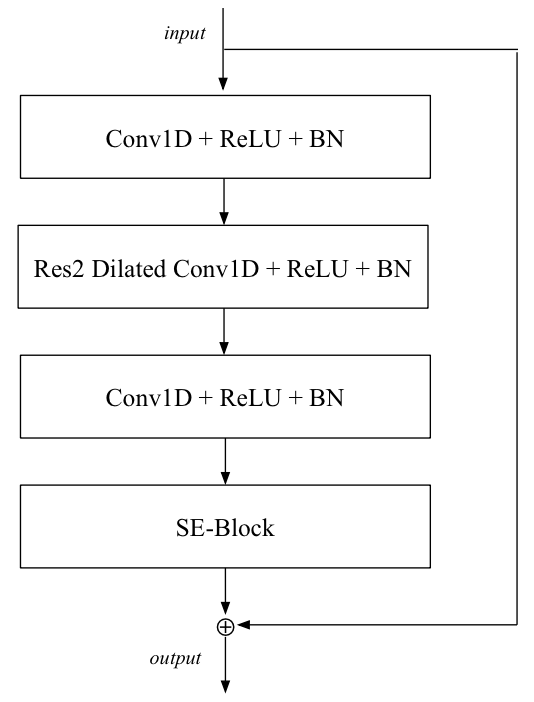
\includegraphics[width=0.42\textwidth]{img/se_res2block_ecapa.png}
\caption{SE-Res2Block of ECAPA-TDNN \cite{ecapa-tdnn}.}
\label{fig:se-res2block}
\end{figure}

\subsubsection{Full Architecture}

As shown in Figure~\ref{fig:ecapa-full}, 80-dimensional Mel filterbank features pass through an initial Conv1D ($k\!=\!5$), followed by three SE-Res2Blocks with increasing dilation ($d = 2, 3, 4$). The residual connection for each block is defined as the sum of \emph{all} preceding block outputs, not just the immediate input.

The outputs of all three blocks are concatenated (\textbf{multi-layer feature aggregation}) and fused by a Conv1D ($k\!=\!1$) into $1536 \times T$ features. A \textbf{channel-dependent attentive statistics pooling} layer computes per-channel attention weights---augmented with a global context vector (utterance-level mean and standard deviation)---to produce weighted means and standard deviations ($3072 \times 1$). A final FC layer yields a 192-dim embedding, trained with AAM-Softmax \cite{deng2019arcface}.

\begin{figure}[H]
\centering
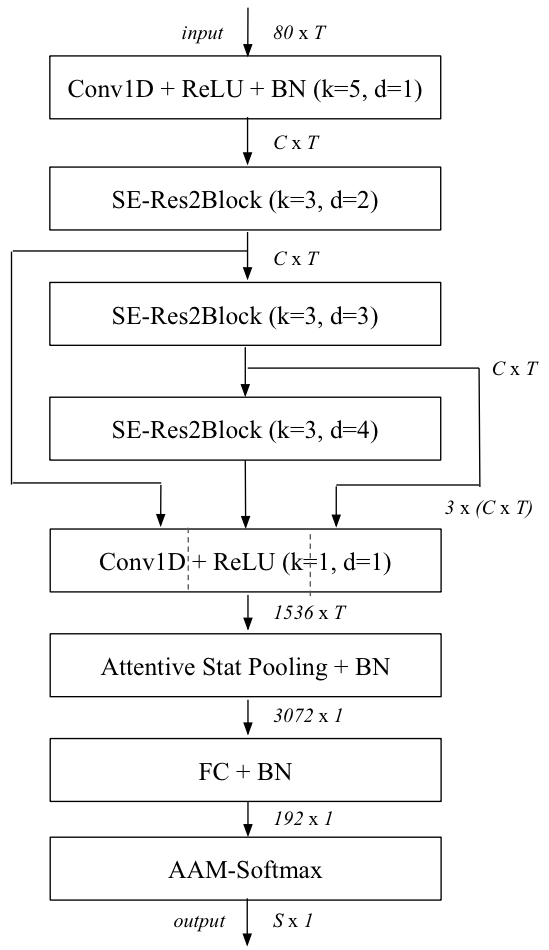
\includegraphics[width=0.52\textwidth]{img/full_ecapa.png}
\caption{Full ECAPA-TDNN architecture \cite{ecapa-tdnn}.}
\label{fig:ecapa-full}
\end{figure}

\subsection{RawNet3}

RawNet3, proposed by Jung et al.\ \cite{rawnet3}, is the third generation of the RawNet family \cite{rawnet, rawnet2}. It adopts ECAPA-TDNN's macro-topology but replaces the handcrafted front-end with a learnable one and adapts the building blocks for raw waveform input.

\subsubsection{AFMS-Res2MP-Block}

The backbone block (Figure~\ref{fig:afms-res2mp}) mirrors the SE-Res2Block with two modifications. First, \textbf{max pooling} is applied after the residual addition to reduce the much longer raw waveform sequences (pool sizes $p = 5$ and $p = 3$ in the first two blocks, while the third block applies no max pooling which is equivalent to $p = 1$). Second, \textbf{Adaptive Feature Map Scaling (AFMS)}---inherited from RawNet2---replaces the SE module, applying a learned affine channel-wise transformation based on global statistics.

\begin{figure}[H]
\centering
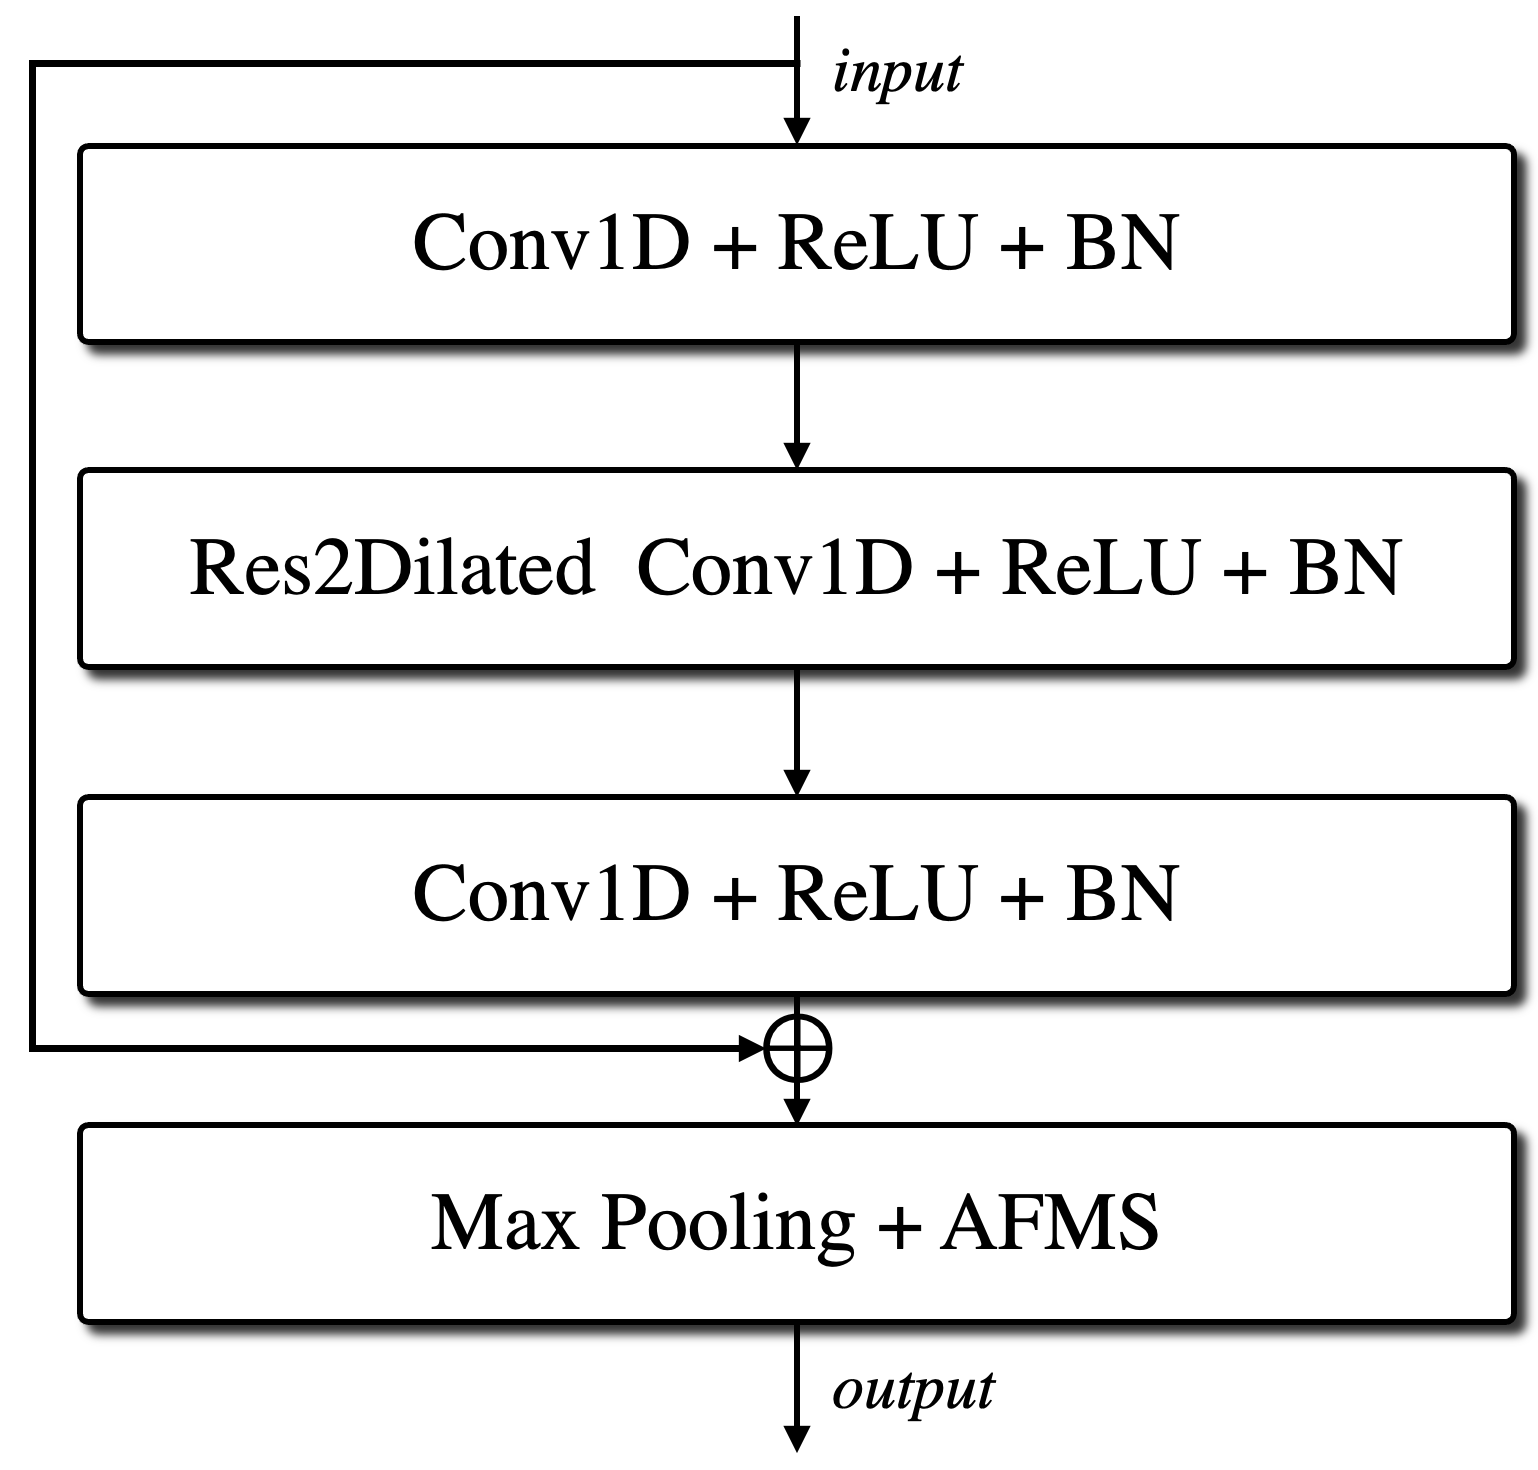
\includegraphics[width=0.45\textwidth]{img/afms-res2mp-rawnet3.png}
\caption{AFMS-Res2MP-block of RawNet3 \cite{rawnet3}.}
\label{fig:afms-res2mp}
\end{figure}

\subsubsection{Full Architecture}

As shown in Figure~\ref{fig:rawnet3-full}, raw waveforms ($1 \times T$) first pass through pre-emphasis, instance normalization, and a \textbf{parameterized analytic filterbank}---a learnable Conv1D ($k\!=\!251$, stride $S$) that replaces fixed acoustic-feature extraction, followed by log compression and mean normalization.

Three AFMS-Res2MP-blocks with parameters $(k, d, p) = (3,2,5),\; (3,3,3),\; (3,4,1)$, where $p=1$ denotes no effective temporal downsampling in the third block. Following ECAPA-TDNN, all block outputs are concatenated and fused by a Conv1D. \textbf{Channel and context statistics pooling} (replacing RawNet2's GRU) collapses the temporal axis into $3072 \times 1$. A FC layer produces a 256-dim embedding, trained with AAM-Softmax.

\begin{figure}[H]
\centering
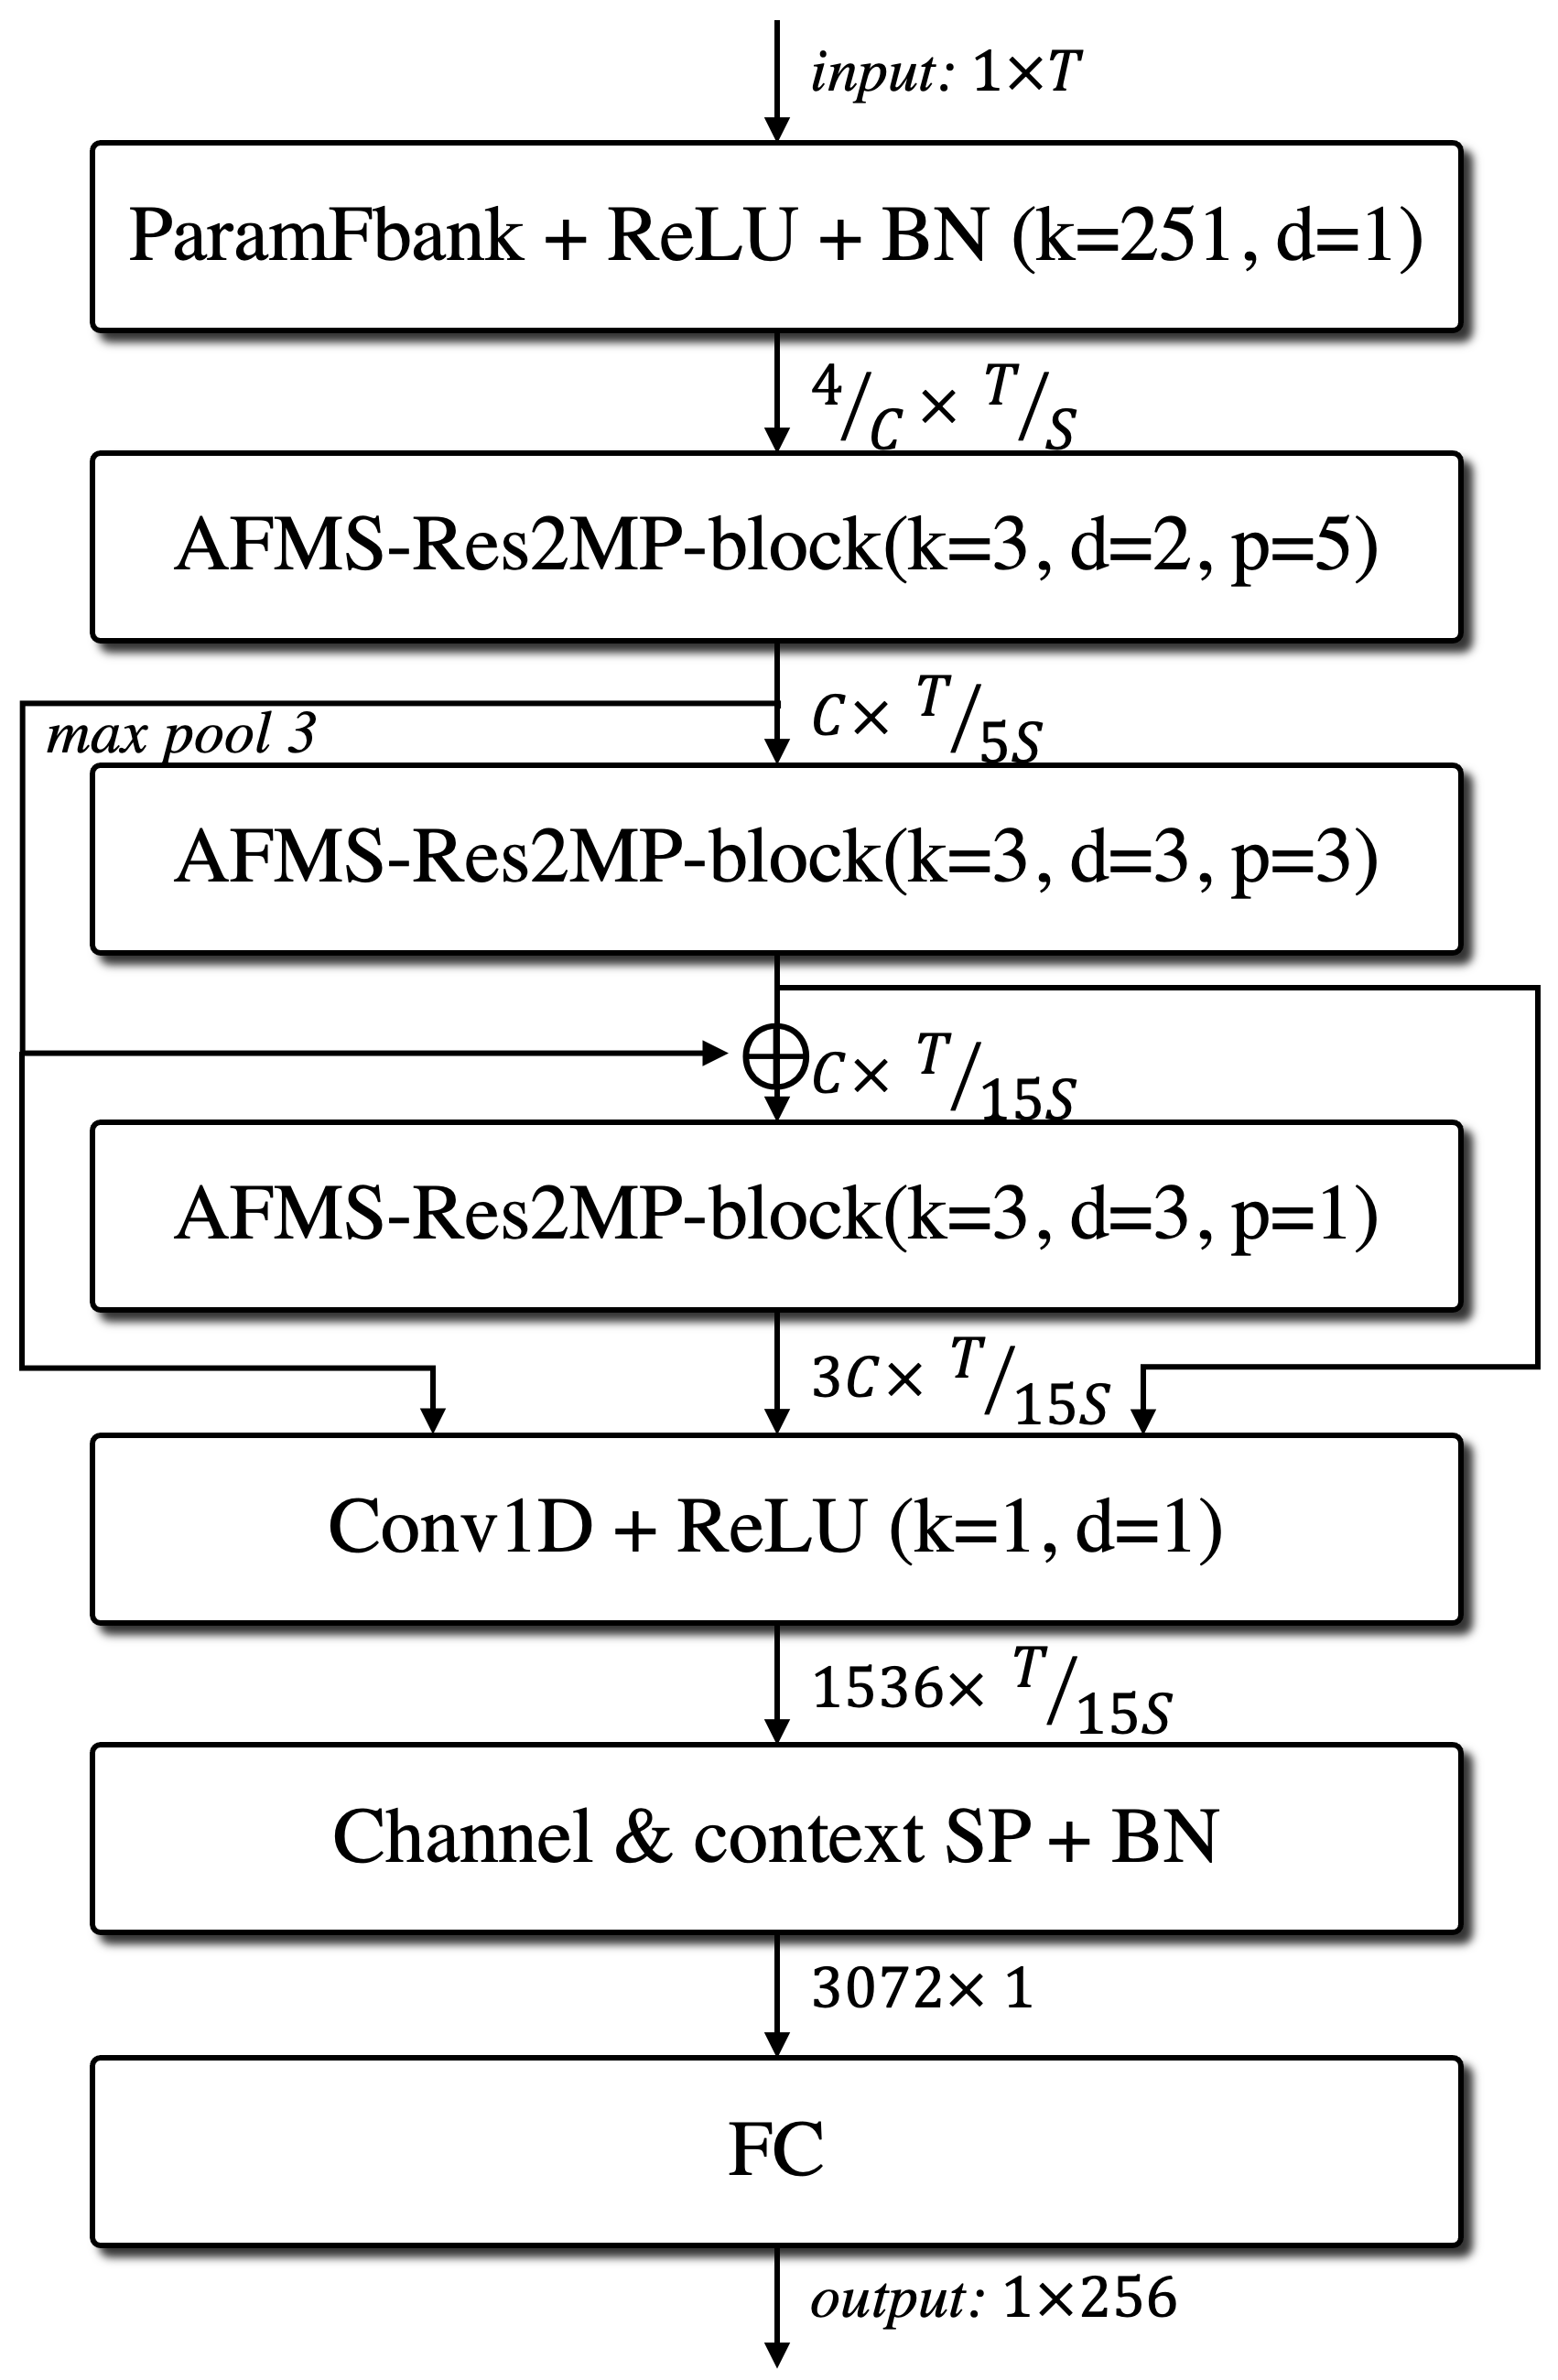
\includegraphics[width=0.52\textwidth]{img/rawnet3_full.png}
\caption{Full RawNet3 architecture \cite{rawnet3}.}
\label{fig:rawnet3-full}
\end{figure}

\subsection{Architectural Comparison}

\begin{table}[H]
\centering
\begin{tabular}{lll}
\toprule
\textbf{Property} & \textbf{ECAPA-TDNN} & \textbf{RawNet3} \\
\midrule
Input               & 80-dim Mel Featurebank feature & Raw waveform \\
Front-end           & Fixed (handcrafted)            & Learned (analytic fbank) \\
Core block          & SE-Res2Block                   & AFMS-Res2MP-block \\
Channel attention   & Squeeze-Excitation             & AFMS \\
Sequence reduction  & ---                            & Max pooling \\
Pooling             & Channel-dep.\ ASP              & Channel \& context SP \\
Embedding dim       & 192                            & 256 \\
\bottomrule
\end{tabular}
\caption{Comparison of ECAPA-TDNN and RawNet3.}
\label{tab:model-comparison}
\end{table}
